\documentclass[a4paper,12pt]{article}
\usepackage[a4paper,top=1.3cm,bottom=2cm,left=1cm,right=1cm,marginparwidth=0.75cm]{geometry}

\usepackage{mathtext} 
\usepackage{setspace}
\usepackage{tabularx}
\usepackage{cmap}
\usepackage{longtable}
\usepackage{icomma}
\usepackage{euscript}
\usepackage{float}
\usepackage{cutwin}
\usepackage{mathrsfs}
\usepackage{adjustbox}
\usepackage{dashbox}
\usepackage[normalem]{ulem}
\usepackage[T1,T2A]{fontenc}	
\usepackage[utf8]{inputenc}         
\usepackage[english,russian]{babel} 
\usepackage[babel=true]{microtype}
\RequirePackage[T1]{fontenc}
\usepackage{amsmath,amsfonts,amssymb,amsthm,mathrsfs,mathtools} 
\usepackage{xcolor}         
\usepackage{enumitem}     
\usepackage{xpatch}       
\usepackage{cancel}                  
\usepackage{upgreek}                 
\usepackage{lipsum}                  
\usepackage[version=4]{mhchem}       
\usepackage{multirow}                
\usepackage{stackengine}             
\usepackage{tikz}         
\usepackage{hyperref}
\hypersetup{colorlinks=true,urlcolor=blue}       
\usetikzlibrary{positioning}         
\usepackage{titletoc}                
\usepackage{titlesec}                
\usepackage{wrapfig}                 
\usepackage{chngcntr}              
\usepackage{fancyhdr}                
\usepackage{makecell}                
\usepackage{indentfirst}             
\usepackage{tocloft}                 
\usepackage{soul}                   
\usepackage[stable]{footmisc}       
\usepackage{subfig}                  

\mathtoolsset{showonlyrefs=true}


\theoremstyle{definition}
\newtheorem*{definition}{Определение}
\newtheorem{statement}{Предложение}[section]
\newtheorem{lemma}{Лемма}[section]
\newtheorem{theorem}{Теорема}[section]
\newtheorem*{theoremn}{Теорема}
\newtheorem*{corollary}{Следствие}
\newtheorem*{example}{Пример}
\newtheorem*{note}{Замечание}
\newtheorem*{problem}{Задача}


\counterwithout{footnote}{section}\DeclareRobustCommand{\divby}{%
	\mathrel{\text{\vbox{\baselineskip.65ex\lineskiplimit0pt\hbox{.}\hbox{.}\hbox{.}}}}%
}

\newcommand{\dotpr}[2]{\bra{#1}\ket{#2}}
\let\AA\relax
\let\emptyset\varnothing
\DeclareMathOperator*{\esssup}{ess sup}
\DeclareMathOperator*{\ord}{ord}
\DeclareMathOperator*{\supp}{supp}
\DeclareMathOperator*{\pr}{pr}
\DeclareMathOperator*{\Ker}{Ker}
\DeclareMathOperator*{\Vol}{Vol}
\DeclareMathOperator*{\rg}{rk}
\DeclareMathOperator*{\Ima}{Im}
\DeclareMathOperator*{\Alt}{Alt}
\DeclareMathOperator*{\Sym}{Sym}
\newcommand{\eqdef}{\stackrel{\text{\tiny{def}}}{=}}
\newcommand{\pp}{\partial}
\newcommand{\AA}{\mathcal{A}}
\newcommand{\BB}{\mathcal{B}}
\newcommand{\MM}{\mathbb{M}}
\newcommand{\NN}{\mathbb{N}}
\newcommand{\ZZ}{\mathbb{Z}}
\newcommand{\QQ}{\mathbb{Q}}
\newcommand{\RR}{\mathbb{R}}
\newcommand{\CC}{\mathbb{C}}
\newcommand{\FFF}{\mathbb{F}}
\newcommand{\DD}{\mathcal{D}}
\newcommand{\FF}{\mathcal{F}}
\newcommand{\sS}{\mathcal{S}}
\newcommand*\circled[1]{\tikz[baseline=(char.base)]{
		\node[shape=circle,draw,inner sep=2pt] (char) {#1};}}


\documentclass[a4paper,12pt]{article}
\usepackage[a4paper,top=1.3cm,bottom=2cm,left=1cm,right=1cm,marginparwidth=0.75cm]{geometry}

\usepackage{mathtext} 
\usepackage{setspace}
\usepackage{tabularx}
\usepackage{cmap}
\usepackage{longtable}
\usepackage{icomma}
\usepackage{euscript}
\usepackage{float}
\usepackage{cutwin}
\usepackage{mathrsfs}
\usepackage{adjustbox}
\usepackage{dashbox}
\usepackage[normalem]{ulem}
\usepackage[T1,T2A]{fontenc}	
\usepackage[utf8]{inputenc}         
\usepackage[english,russian]{babel} 
\usepackage[babel=true]{microtype}
\RequirePackage[T1]{fontenc}
\usepackage{amsmath,amsfonts,amssymb,amsthm,mathrsfs,mathtools} 
\usepackage{xcolor}         
\usepackage{enumitem}     
\usepackage{xpatch}       
\usepackage{cancel}                  
\usepackage{upgreek}                 
\usepackage{lipsum}                  
\usepackage[version=4]{mhchem}       
\usepackage{multirow}                
\usepackage{stackengine}             
\usepackage{tikz}         
\usepackage{hyperref}
\hypersetup{colorlinks=true,urlcolor=blue}       
\usetikzlibrary{positioning}         
\usepackage{titletoc}                
\usepackage{titlesec}                
\usepackage{wrapfig}                 
\usepackage{chngcntr}              
\usepackage{fancyhdr}                
\usepackage{makecell}                
\usepackage{indentfirst}             
\usepackage{tocloft}                 
\usepackage{soul}                   
\usepackage[stable]{footmisc}       
\usepackage{subfig}                  

\mathtoolsset{showonlyrefs=true}



\counterwithout{footnote}{section}\DeclareRobustCommand{\divby}{%
	\mathrel{\text{\vbox{\baselineskip.65ex\lineskiplimit0pt\hbox{.}\hbox{.}\hbox{.}}}}%
}




\title{Измерение коэффициента поверхностного натяжения жидкости (2.5.1)}
\author{Дудаков Семён}
\date{\today}


\begin{document}
	\maketitle
	\section{Аннотация}
	В данной работе мы находим коэффициент поверхностного натяжения, с помощью иглы, колб с жидкостями и аспиратора, создающего разность давления.
	\section{Введение}
	\noindent\textbf{Цель работы:}
	1) измерение температурной зависимости  коэффициента поверхностного натяжения дистиллированной воды с использованием известного коэффициента поверхностного натяжения спирта; 2) определение полной поверхностной энергии  и теплоты, необходимой для изотермического образования единицы  поверхности жидкости  при различной температуре.
	
	\bigskip
	\noindent\textbf{В работе используются:} прибор  Ребиндера  с термостатом и микроманометром; исследуемые жидкости; стаканы; микроскоп.
	\section{Теоретические сведения}
	
	Наличие поверхностного слоя приводит к различию давлений по разные стороны от искривленной границы раздела двух сред.  Для сферического пузырька с воздухом  внутри жидкости избыточное давление дается формулой Лапласа:
	
	\begin{equation}
		\Delta P = P_{int} - P_{ext} = \frac{2\sigma}{r},
		\label{key}
	\end{equation}
	где $ \sigma $ -- коэффициент поверхностного натяжения, $ P_{int} $ и $ P_{ext} $ -- давление внутри пузырька и снаружи, $ r $ -- радиус кривизны поверхности раздела двух фаз. Эта формула лежит в основе предлагаемого метода определения коэффициента поверхностного натяжения жидкости. Измеряется давление $ \Delta P $, необходимое для выталкивания в жидкость пузырька воздуха.
	
	\section{Экспериментальная установка}
	
	\begin{wrapfigure}{R}{6cm}
		%\vspace{-61pt}
		\begin{center}
			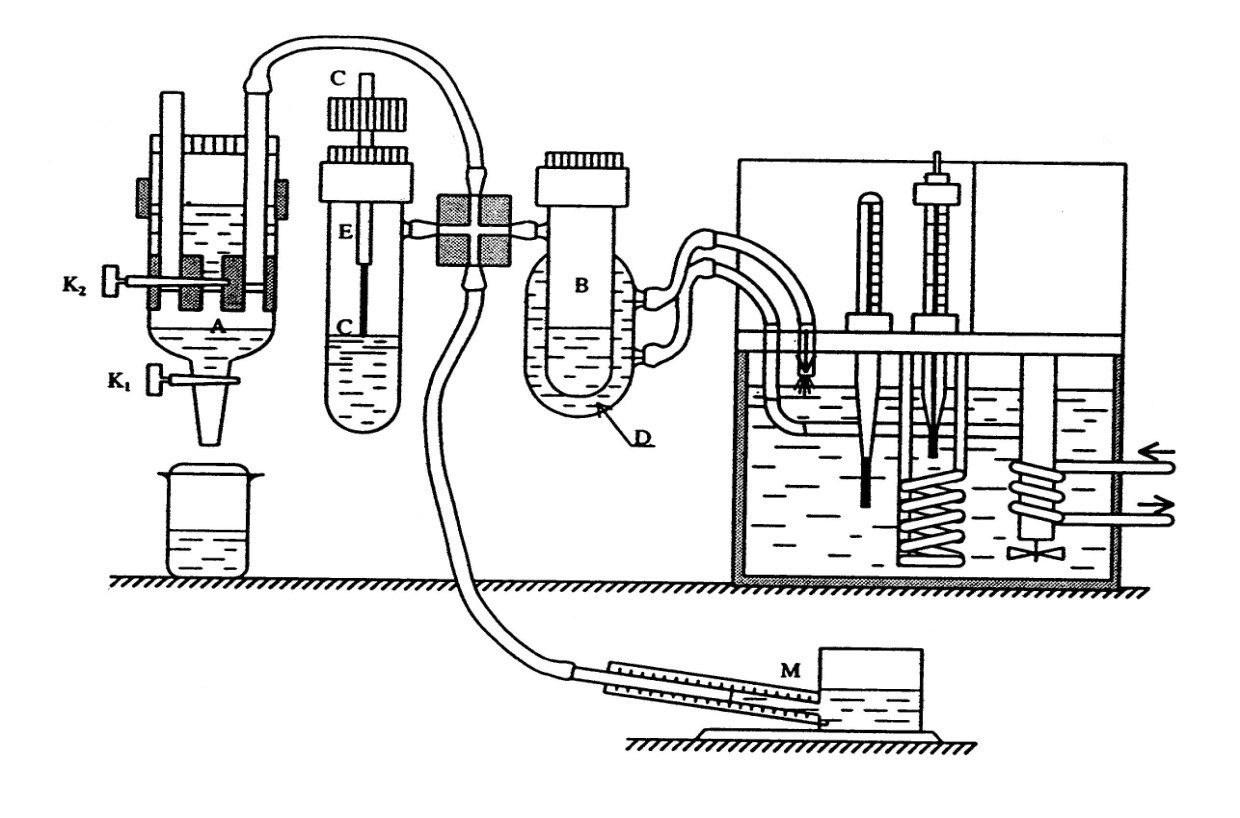
\includegraphics[width=5.9cm]{fac.jpg}
			\caption{Рисунок экспериментальной установки}
			\label{img:ust}
		\end{center}
	\end{wrapfigure}
	
	Исследуемая жидкость (дистиллированная вода) наливается в сосуд (колбу) $ B $ (рис. \eqref{img:ust}). Тестовая жидкость  (этиловый спирт) наливается  в сосуд $ E $.  При измерениях  колбы герметично закрываются  пробками. Через одну из двух пробок  проходит полая металлическая игла $ С $. Этой пробкой закрывается сосуд, в котором  проводятся измерения. Верхний конец иглы открыт в атмосферу, а нижний погружен в жидкость. Другой сосуд герметично закрывается второй пробкой. При создании достаточного  разряжения воздуха в колбе с иглой пузырьки воздуха начинают пробулькивать через жидкость. Поверхностное натяжение можно определить по величине разряжения $ \Delta P $ \eqref{key}, необходимого для прохождения пузырьков (при известном радиусе иглы).
	
	Разряжение в системе создается с помощью аспиратора $ A $. Кран $ K_2 $ разделяет две полости аспиратора. Верхняя полость при закрытом кране $ K_2 $ заполняется водой. Затем кран $ K_2 $ открывают и заполняют водой  нижнюю полость  аспиратора.  Разряжение воздуха создается в нижней полости  при открывании крана $ K_1 $, когда  вода вытекает из неё по каплям. В колбах $ В $ и $ С $, соединённых трубками с нижней полостью аспиратора, создается такое же пониженное давление. Разность давлений в полостях с разряженным воздухом и атмосферой измеряется спиртовым микроманометром. 
	
	Для стабилизации температуры исследуемой жидкости через рубашку $ D $ колбы $ В $ непрерывно прогоняется вода из термостата.
	
	Обычно кончик иглы лишь касается поверхности жидкости, чтобы исключить влияние гидростатического давления столба жидкости. Однако при измерении температурной зависимости коэффициента поверхностного натяжения возникает ряд сложностей. Во-первых, большая теплопроводность металлической трубки приводит к тому, что температура на конце трубки заметно ниже, чем в глубине жидкости. Во-вторых, тепловое расширение поднимает уровень жидкости при увеличении температуры.
	
	Обе погрешности можно устранить, погрузив кончик трубки до самого дна. Полное давление, измеренное при этом микроманометром, равно \[ P = \Delta P + \rho g h.\] Заметим, что $ \rho gh $ от температуры практически не зависит, так как подъём уровня жидкости компенсируется уменьшением её плотности (произведение $ \rho g $ определяется массой всей жидкости и поэтому постоянно). Величину  $ \rho g h $ следует измерить двумя способами.
	
	Во-первых, замерить величину $ P_1= \Delta P' $, когда кончик трубки только касается поверхности жидкости. Затем при этой же температуре опустить иглу до дна и замерить $ P_2= \rho gh + \Delta P'' $ ($ \Delta P' $, $ \Delta P'' $ -- давление Лапласа). Из-за  несжимаемости  жидкости можно положить $ \Delta P' = \Delta P'' $ и тогда \[ \rho gh= P_2 - P_1. \]
	
	Во-вторых, при измерениях $ P_1 $ и $ P_2 $ замерить линейкой  глубину погружения иглы $ h $. Это можно сделать, замеряя расстояние между верхним концом иглы и любой неподвижной частью прибора при положении иглы на поверхности и в глубине колбы.
\newpage
	
	\section{Ход работы}
 \subsection{Измерение диаметра иглы}
	Измерим максимальное давление при пробулькивании пузырьков воздуха через спирт:
	\begin{table}[H]
		\begin{center}
			\begin{tabular}{|c|c|c|c|}
				\hline
				$P_\text{спирт}$, мм&44&45&46\\
				\hline
				$P^{\text{ср}}_\text{спирт}$, мм& \multicolumn{3}{|c|}{45}\\
                \hline
			\end{tabular}
		\end{center}
		\caption{Результаты измерений в спирте}
		\label{tab1}
	\end{table}

    $\sigma_P = \sqrt{\left(\sigma_P^\text{сист}\right)^2 + \left(\sigma_P^\text{случ}\right)^2} = \sqrt{2^2 + 0.8^2} \approx 2$
 
	По формуле \eqref{key} найдем диаметр иглы:
	\begin{equation*}
		d = \frac{4\sigma_{\text{с}}}{P^{\text{ср}}_\text{спирт}Kg} = (1.00\pm 0.04)\text{ мм}, \varepsilon_r = 4\%
	\end{equation*}

	Результат полученный под микроскопом: $D = (1,00\pm0.05)$ мм, $\varepsilon_r = 5\%$ это означает, что диаметр найденный экспериментально достаточно точен.
	
	\subsection{Измерение температурной зависимости коэффициента поверхностного натяжения}
	
	Снимать будем двумя способами: при касании поверхности воды и при полном погружении иглы.
	
	Глубина погружения измеренная линейкой: $\Delta h = (1.6\pm0.2)$ см, $\varepsilon_{\Delta h} = 13\%$. Глубина погружения по разнице давлений из первого опыта: $\Delta P = (211-148)*0.2*9.81 = 123.6\pm3,9$ Па, $\varepsilon_{\Delta P} = 3,2\%$, $\Delta h = \dfrac{\Delta P}{\rho g} = (1.56\pm0.05)$ см, $\varepsilon_{\Delta h} = 3,2\%$.
	
	Внесём все измеренные и полученные данные в таблицу:
    \begin{table}[H]
            \centering
            \begin{tabular}{|c|c|c|c|c|c|c|c|c|}
            \hline
            $T$, \textdegree C   & $P$, мм   & $\sigma$, мН/м &$\Delta\sigma$, мН/м & $\varepsilon_{\Delta \sigma}$ &$q$, мН/м    & $\Delta q$, мН/м  & $U/\Pi$, мН/м & $\Delta (U/\Pi)$, мН/м \\ \hline
            24.9 & 211 & 72.6  & 1 & 1.4 & 3.9 & 0.16 & 76.5 & 1.1  \\ \hline
            30.5 & 210 & 72.1  & 1  & 1.4 & 4.7 & 0.2 & 76.8 & 1.2  \\ \hline
            35.5 & 208 & 71.1  & 1   & 1.4 & 5.5 & 0.23 & 76.6 & 1.1  \\ \hline
            40.5 & 206 & 70.1 & 1   & 1.4 & 6.3 & 0.26 & 76.4 & 1.1 \\ \hline
            45.4 & 205 & 69.7  & 1   & 1.4 & 7 & 0.3 & 76.7 & 1.2  \\ \hline
            50.5 & 203 & 68.7  & 1   & 1.5 & 7.8 & 0.33 & 76.5 & 1.1  \\ \hline
            55.5 & 202 & 68.2  & 1   & 1.5 & 8.6 & 0.36 & 76.8 & 1.2  \\ \hline
            59.8 & 200 & 67.2  & 1   & 1.5 & 9.3 & 0.39 & 76.5 & 1.1  \\ \hline
            \end{tabular}
            \caption{Зависимости $\sigma(T)$, $q(T)$ и $U/\Pi(T)$}
            \label{table}
    \end{table}
    \newpage
    Строим по ним графики зависимости $\sigma(T)$:

    \begin{figure}[h!]
            \centering
            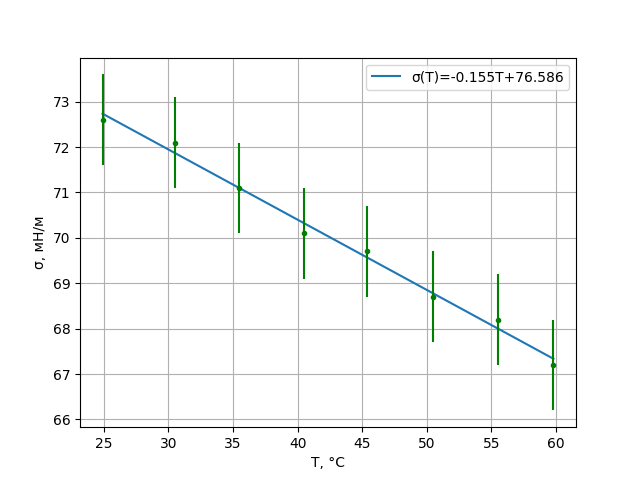
\includegraphics{st.png}
            \caption{График $\sigma(T)$}
            \label{graph}
    \end{figure}
	Температурные коэффициенты:
    \begin{itemize}
	\item $ \displaystyle \underline{k = \frac{d\sigma}{dT} = (-0,155 \pm 0,006) \text{ } \frac{\text{мН}}{\text{м}\cdot\text{К}}, \: (\varepsilon = 4,2\%);} $
	\item $ \displaystyle \underline{b = (76,6 \pm 3,9) \text{ } \frac{\text{мН}}{\text{м}}, \: (\varepsilon = 5,1\%).}$
    \end{itemize}

	\subsection{Графики других величин}
	Окончательно, с помощью полученных данных построим графики теплоты образования единицы поверхности жидкости: $q = - T\cdot\dfrac{d\sigma}{dT}$ и поверхностной энергии $U$ единицы площади $\Pi$: $\dfrac{U}{\Pi} = \sigma - T\cdot\dfrac{d\sigma}{dT}$.
 \newpage
    \begin{figure}[h!]
            \centering
            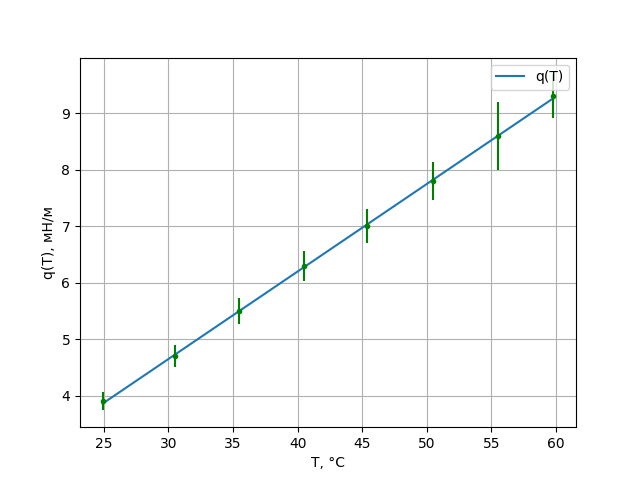
\includegraphics[scale=0.9]{qt.png}
            \caption{График $q(T)$}
            \label{graph}
    \end{figure}
    \begin{figure}[h!]
            \centering
            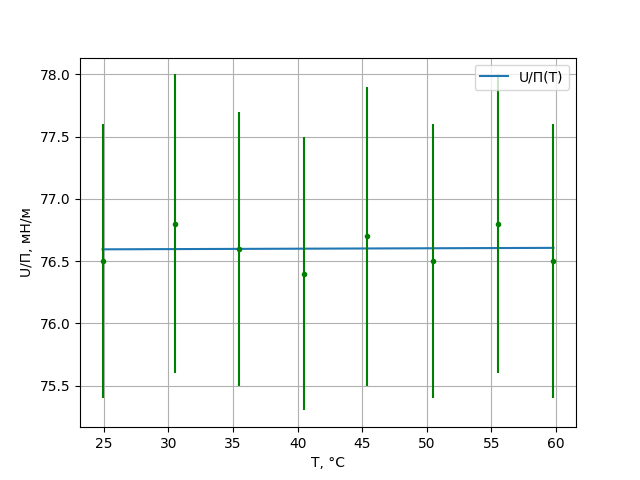
\includegraphics[scale=0.9]{ut.png}
            \caption{График $U/П(T)$}
            \label{graph}
    \end{figure}
    \begin{figure}[h!]
            \centering
            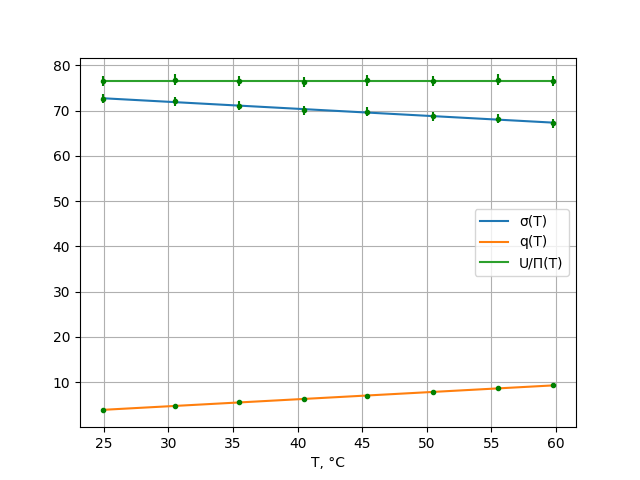
\includegraphics[scale=0.9]{all.png}
            \caption{График $U/П(T)$}
            \label{graph}
    \end{figure}
\newpage
	\section{Вывод}
	В ходе работы:
	\begin{enumerate}
		\item Был экспериментально измерен диаметр иглы при помощи коэффициента поверхностного натяжения спирта. Полученный результат $d = (1.00\pm 0.04)\text{ мм}$ с достаточной точность совпадает с диаметром измеренным с помощью микроскопа.
		\item Было измерено давление, создаваемое столбом жидкости при опускании иглы на $\Delta h = (1.6\pm 0.2)$ см.
		\item Получены коэффициенты поверхностного натяжения воды при различных ее температурах, например $\sigma = (72.6\pm 1)\:\frac{\text{мН}}{\text{м}}$ при температуре 25 $^\circ$С.
		\item Были построены графики зависимости различных величин от температуры.
	\end{enumerate}

\end{document}
